\documentclass[output=paper]{langsci/langscibook}
\author{Mary Aizawa Kato\affiliation{Universidade Estadual de Campinas}\and
Maria Eugenia L. Duarte\affiliation{Universidade Federal do Rio de Janeiro}}
\title{Parametric variation: The case of Brazilian Portuguese null subjects}

% \chapterDOI{} %will be filled in at production

\abstract{This chapter revisits comparative and diachronic studies of linguists
    analysing Brazilian Portuguese (BP) with regard to the NSP, especially in view
    of recent debates on the existence of the so-called Partial Null Subject
    languages. It will be shown that BP is losing the properties of a
    prototypical NSL like European Portuguese (EP), with a rich inflectional
    paradigm, but, as the change is very recent, there is still not a consensus
    regarding the target of the change. Our question is whether BP classifies
    as a PNS language like Finnish, Hebrew or Marathi, as was recently claimed
    in \textcite{Holmberg2010}, and \textcite{HolShee2010}. Methodologically,
    it is our purpose to observe the overt and null subjects in real data so as
    to check whether eventual optionality of null and overt pronouns can be
    attributed to a grammatical competition from a diachronic perspective
    \parencite{Kroch1994} or to some licensing possibility within a single type
    of grammar, which is normally a view taken by formal linguists analyzing
    synchronic data. Using acquisition\is{language acquisition} data we will show that while null
    non-referential subjects are part of Brazilian \isi{core grammar}, null
    referential subjects are not, and their existence in the production of
    Brazilian literate adults results from instruction through schooling. The
    chapter suggests that from a typological view BP is a semi-NS language like
Icelandic.}

\maketitle

\begin{document}\glsresetall

\section{The Null Subject Parameter: A background}

Since the advent of the Principles and Parameters model within the Government
and Binding theory (\citealt{Chomsky1981,Rizzi:1982}, a.o), the \gls{NSP} has
received the widest range of discussions and refinements.  Not only did its
formal formulation deserve a lot of attention, but its typological binary
concept (\citealt{Chomsky1981}, based on \citealt{Taraldsen1978}) gave rise to
a new way to do comparative and historical linguistics.  But
\citet[144]{Rizzi:1982} soon pointed to the fact that what was considered a
single parameter should be decomposed into two sub-parameters,\is{parameters} distinguishing
languages allowing both null referential and expletive\is{expletives} subjects from those
licensing only null expletives (what he calls \emph{semi-pro-drop}
languages)\footnote{Which we will later call semi-[non-NS] languages, after
\citet{Biberauer2010}.} (e.g.: \ili{Italian} vs.\ German).

Further studies in the 1980s and 1990s would show that morphological
richness\footnote{“The intuitive idea is that where there is overt agreement,
the subject can be dropped, since the deletion is recoverable”
\parencite[241]{Chomsky1981}.} was not sufficient to explain licensing and
identification of null subjects. \citegen{Huang1984} classical article showed
that null subjects were also licensed in systems like Chinese, without any
inflection for mood, tense, number and person, which led to a new hypothesis
(\citet{JaeggliSafir1989}, according to which what licenses null subjects is
not a “rich” inflectional verbal paradigm but its morphological uniformity.  In
the case of a paradigm consisting of different affixes, identification would
occur through agreement marks; in the case of a paradigm consisting of a single
stem, identification would be possible through a discursive topic. In the first
case the NS would be a pronominal category; in the second, a variable. If,
however, a paradigm is mixed, the NS would not be licensed.

\citet{Roberts1993} would bring new contributions to the discussion based on
diachronic evidence from medieval \ili{French}. He argued that a “functionally” rich
paradigm, i.e.\ with a zero ending and two identical forms for different
grammatical persons, could act as a “formally” rich one. The author, however,
pointed out the fact that the limit of syncretic forms could not be
exceeded. This proposal has been used to explain licensing of null subjects in
European Portuguese and Brazilian Portuguese before the latter underwent a
change in its inflectional paradigm, as we will show in \Cref{sec:key:26.2.2}.

The cluster of properties, which has been crucially related to the \gls{NSL}\is{null subject languages}
since the classical formulation of the \gls{NSP}, has not been thoroughly
confirmed in more than thirty years of research, which has led to negative
conclusions and certain scepticism with respect to the Principles and
Parameters Theory, according to \citet{RobHol2010}.

\glsunset{PNS} In recent years, in the light of new theoretical and empirical
evidence, the notion of “partially” null subject (\gls{PNS}) languages has been
introduced (cf.\ \citealt{Holmberg2005}; works in
\citealt{Biberauer2008,BibHolRobShee2010}, a.o.), which draws a much more
complex picture, leading to a proposal of \isi{parameter hierarchies}, able to
accommodate different parametric values. The representation in \eqref{ex:key:26.1},
still covering languages with some sort of agreement, includes such \gls{PNS}\is{null subject languages!partial null subject languages}
systems (cf.\ \citealt{HolShee2010}; \citealt[6]{Sheehan2014b}, a.o.):

\ea%1
    \label{ex:key:26.1}
    \hspace*{-1.0cm}
    \begin{tikzpicture}[baseline=(root.base), align=center, font=\small]

        \Tree 	[.\node(root){Is INFL [$+$pronoun]?};
                    {No\\\emph{overt subject}}
                    [.\node(y1){Yes:};
                        {No\\\emph{expletive \emph{pro}}}
                        [.\node(y2){Yes:};
                            {Yes\\\emph{referential \emph{pro}}}
                            [.\node(y3){No:};
                                {Yes\\\emph{partial NS}}
                                {No\\\emph{\emph{quasi}-argumental \emph{pro}}}
                            ]
                        ]
                    ]
                ]

        \node [right=1.5mm of y1.east] {Is INFL [$+$pronoun] referential?};
        \node [right=1.5mm of y2.east] {Is INFL [$+$person]?};
        \node [right=1.5mm of y3.east] {Can INFL be bound?};

    \end{tikzpicture}
\z

Based on evidence coming from a number of languages of different families,
\citeauthor{RobHol2010} list, beside non-null subject languages,\footnote{We
    must keep in mind that non-null subject languages do not admit null
    subjects in neuter contexts. We do not ignore the fact that such
systems can exhibit null subjects, pragmatically identified in non-neuter
contexts (see, for instance, null 1st person subjects in \ili{English} diaries,
\citealt{Haegeman1990}).} the following types of \glspl{NSL}: consistent
\glspl{NSL}, such as \ili{Italian}, \ili{Greek} and \ili{Turkish}, with “rich”
inflection; null expletive\is{expletives} languages (also referred as \emph{semi}
\emph{pro-drop}), which do not allow referential NSs, among which we can find
\ili{German} and some varieties of \ili{Dutch} and many creoles, as
\ili{Capeverdian}, \ili{Haitian}, and \ili{Jamaican}; radical null
subject\is{null subject languages!radical null subject languages}
languages (\emph{discourse pro-drop}), as Chinese, \ili{Japanese} and
\ili{Thai}, with no agreement mark, which allow null subjects and objects in
appropriate discursive conditions; and finally, partial null subject languages,
including \ili{Finnish}, \ili{Hebrew}, \ili{Icelandic}, \ili{Russian},
\ili{Marathi} (a variety spoken in western India) and \ili{Brazilian
Portuguese}.  According to the authors, they constitute a more difficult type
to define because the languages under such label may show a range of
characteristics too diverse. \gls{BP}\il{Brazilian Portuguese}, on the
contrary, instead of creating a lexical expletive\is{expletives} like \ili{French}, shows a
competition between a null subject, and a prominent constituent moved to the
structural subject position, resembling constructions of discourse
configurational languages.

The proposal of \isi{parameter hierarchies} can be related to the notion of
\emph{micro}-parameters\is{parameters} \citep{Kayne1996}, which could explain small
differences among similar systems. According to \citet{Roberts2012}, each
formal feature defines a distinct parameter, and he also argues that parameters
move from “macro” to “micro” levels; thus, it would be natural to expect lower
layers in the hierarchy to become more marked, showing a more complex behaviour
than upper layers. The relevance of the parameter hierarchy\is{parameter
hierarchies} for acquisition\is{language acquisition}
should be the prediction that higher options would be preferred as they are
less marked; as more marked options appear in the primary data, the learner
moves to lower levels, until the definition of a parametric setting compatible
with the data is accomplished. The distinction between \emph{micro-} and
\emph{macro}-parameters\is{parameters} would not be, according to \citet[310]{Roberts2012},
part of \gls{UG}\is{Universal Grammar}, but a property that emerges as a result of the interaction of the
learner with the primary data and \gls{UG}\is{Universal Grammar}. These hierarchies also include some
predictions about diachronic changes: they should happen in the direction of
upper hierarchies, less marked, driven by functional pressures or linguistic
contact.

Finally, refining \eqref{ex:key:26.1}, \textcite{RobHol2010} proposed the \gls{NSP}
hierarchy in \eqref{ex:key:26.2}, suggesting that each functional head\is{functional items} defines its
parametric hierarchy:

\ea%2
    \label{ex:key:26.2}
    \hspace*{-.75cm}%
    \begin{tikzpicture}[baseline=(a.base),%
                        level distance=50pt,%
                        sibling distance=-50pt,%
                        font=\small]
        \tikzset{level 4/.style={sibling distance=5pt}}

        \Tree   [.\node(a){\vphantom{Y}\\a.};
                    {No\\\emph{Radical pro-drop}}
                    [.\node(b){Yes\\b.};
                        {Yes\\\emph{Pronominal arguments}}
                        [.\node(c){No\\c.};
                            {No\\\emph{Non pro-drop}}
                            [.\node(d){Yes\\d.};
                                {Yes\\\emph{Consistent null subject}}
                                No
                            ]
                        ]
                    ]
                ]

        \node [right=1.5mm of a.south, align=left, anchor=south west]
            {Are uφ-features present on probes?};

        \node [right=1.5mm of b.south, align=left, anchor=south west]
            {Are uφ-features present on all probes?};

        \node [right=1.5mm of c.south, align=right, anchor=south west]
            {Are uφ-features fully specified on some probes?};

        \node [right=1.5mm of d.south, align=right, anchor=south west]
            {Are uφ-features fully specified on T?};

    \end{tikzpicture}
\z

In sum, the attempt to accommodate different hierarchies, keeping the binary
values of each parameter,\is{parameters} is in itself evidence that it is not an easy
enterprise. As for the label \gls{NSP} in the interpretation it has had in the
Theory of Principles and Parameters today, it seems to include several
sub-types of languages, as argued by \citet{Biberauer2010}.  We will see that
\gls{BP}\il{Brazilian Portuguese} exhibits a very peculiar behaviour in this
regard.

\section{Preliminaries}\label{sec:key:26.2}

\subsection{Our aims}\label{sec:key:26.2.1}

The aim of this chapter is to revisit the comparative and diachronic studies of
linguists analysing \gls{BP} with regard to the \gls{NSP}, especially in view
of recent debates on the existence of the so-called \gls{PNS}\is{null subject languages!partial null subject languages} languages.  It is
a well known fact that \gls{BP}\il{Brazilian Portuguese} is losing the
properties of a prototypical \gls{NSL}\is{null subject languages}, like \gls{EP}, with a rich
inflectional paradigm, but, as the change is very recent, there is still not a
consensus regarding the target of the change. Our question is whether
\gls{BP}\il{Brazilian Portuguese} classifies as a \gls{PNS}\is{null subject languages!partial null subject languages} language like
\ili{Finnish}, \ili{Hebrew} or \ili{Marathi}, as was recently claimed in \citet{Holmberg2010},
and \citet{HolShee2010}. Methodologically, it is our purpose to observe
the overt and null subjects in real data so as to check whether eventual
optionality of null and overt pronominals can be attributed to a grammatical
competition from a diachronic perspective \citep{Kroch1994} or to some
licensing possibility within a single type of grammar, which is normally a view
taken by formal linguists analysing synchronic data. Using acquisition\is{language acquisition} data
(\citealt{Magalhaes2003} and \citealt{Kato2011}), we will try to see how the
Brazilian child selects their grammar, and will follow the hypothesis that null
referential subjects in the Brazilian literate adult are not residues of the
old grammar, but the result of instruction through schooling.

Our  upcoming sections are organized as follows:  \Cref{sec:key:26.2.2}.
describes the \gls{BP}\il{Brazilian Portuguese} diachronic facts;
\Cref{sec:key:26.2.3} brings some considerations on acquisition\is{language acquisition} data;
\Cref{sec:key:26.3} contains a comparative analysis of \gls{BP}\il{Brazilian
Portuguese} with four types of languages: \Cref{sec:key:26.3.1} with
\gls{EP}\il{European Portuguese}, a consistent \gls{NSL}\is{null subject languages}, with rich Agr
inflection; \Cref{sec:key:26.3.2} with Japanese, a radical type,\is{null subject languages!radical null subject languages} or a discourse
configurational language type, with no Agr inflection; \Cref{sec:key:26.3.3}
with Finnish, a Partial \gls{NSL}\is{null subject languages}; \Cref{sec:key:26.3.4} with \ili{English}, a
[−NS] language; and \Cref{sec:key:26.3.5} with \ili{Icelandic}, the so-called
\emph{semi[NS]} language.

In the conclusions we will summarize the findings of the article, namely that
\gls{BP}\il{Brazilian Portuguese} \isi{core grammar} is set to a [−NS] language with
referential subjects and to a [+NS] language with regard to non-referential
ones.  With regard to the literate Brazilians \isi{E-language} it will be shown to
exhibit a competition with regard to referential subjects, between   overt
pronominal subjects  of the \ili{English} type, and  NSs, of the radical type.\is{null subject languages!radical null subject languages}
With regard to non-referential subjects, the  literate adult maintains the same
types of NSs exhibited by the child.

\subsection{From Old Portuguese to Modern Brazilian
Portuguese}\label{sec:key:26.2.2}

As is well known among Romanists, \gls{OFr}\il{Old French} was “a sort of V2\is{V2 word order}
type of language”  (cf.\ (\ref{ex:key:26.3}a)) and also a \gls{NSL}\is{null subject languages} (cf.\
(\ref{ex:key:26.4}a) (\citealt{Adams1987}, \citealt{Roberts1993}, a.o.). The
latter property was lost when \gls{OFr} lost this characteristic. According to
\citet{Ribeiro1995}, \gls{OP} was also a \gls{NSL}\is{null subject languages} and a “sort of V2\is{V2 word order} type of
language”\footnote{Cf.\ \textcite{Ribeiro1995} for OP and
    \textcite{TorresMoraes1993} for the Classic period.
    Brazilian authors acknowledge that \ili{Romance} V2\is{V2 word order} is not exactly like the
    \ili{Germanic} V2\is{V2 word order}.  See also \citet{Kaiser1999} and \citet{Rinke2009} against Old
    Portuguese as a V2\is{V2 word order} language.}  (cf.\ (\ref{ex:key:26.3}b)).
    \gls{EP}\il{European Portuguese} retained both properties, while
    \gls{BP}\il{Brazilian Portuguese} lost both the same way \gls{OFr} did.

\ea%3
\label{ex:key:26.3}
\ea     \ili{Old French} V2\is{V2 word order}\\
    \gll    Eisint revindrent li mesage     en la ville.\\
            then  returned     the messenger to the town\\
    \glt    ‘Then the messenger returned to town.
    \ex \ili{Old Portuguese} V2\is{V2 word order}\\
    \gll    Maravilhosas \textbf{son} estas cousas que co’ntas, padre\dots\\
            beautiful    are these things   that tell.\Ssg{}, father\\
    \glt    ‘Beautiful are the things that you tell us, father.’
    \z
\z

However, contrary to \ili{Germanic} languages, \gls{OFr} and OP could both exhibit
the V1 pattern (cf.\ \citealt{Kaiser1999}; \citealt{Ribeiro1995}), which in
French was restricted to VS, while in Portuguese it exhibited a null subject:

\ea\label{ex:key:26.4}
\ea     \ili{Old French} V1\\
    \gll    \textbf{Respundi} li evesches.\\
            answered the bishop\\
    \glt    \enquote*{The bishop answered.}
    \ex     \ili{Old Portuguese} V1\\
    \gll    \textbf{Quero} que m’o     digas        e     desejo mui   de coraçon a saber\dots{}\\
            want.\Fsg{} that  me=it tell.\Ssg{} and wish.\Fsg{} much of heart      to know\\
    \glt    \enquote*{I want you to tell me, and I  strongly wish to know...}
    \z
\z

If we take fronted Focus\is{focus} structures (FocusVS) as a diagnosis of V2\is{V2 word order} structures
in older periods of Portuguese, we can say that these started to disappear in
the 18th century in the \gls{BP}\il{Brazilian Portuguese} variety
\parencite{KatoRibeiro2009}. On the other hand, the optionality between NS and
overt pronominal subjects in \gls{BP}\il{Brazilian Portuguese} started to
appear by the end of the 19th century (\citealt{Tarallo1985,Duarte1993}). It is
clear, therefore, that V2\is{V2 word order} structures started to disappear one century before
the NS began to decline, suggesting that the two changes were independent in
\gls{BP}\il{Brazilian Portuguese}, contrary to what has been observed in
\ili{French}.

A number of investigations on the morphosyntax of Brazilian Portuguese point to
the conclusion that variable phenomena have a very regular distribution in the
country. In fact, the polarization to which \citet{Lucchesi2009b} refers to
should be related particularly to variation in the use of agreement marks. The
author himself, in a recent overview of sociolinguistic polarization in Brazil
\parencite{Lucchesi2015}, distinguishes those processes of variation and change
that reach all sectors of Brazilian society \emph{in the same direction} from
those processes which take opposite directions, setting apart high and middle
sectors from those at the base of the social pyramid. In spite of that, the
author himself recognizes a sort of “leveling” towards non-standard variants.

In fact, the alleged contrast may be valid when we consider the rural-urban
\emph{continuum}. Results for contemporary Brazilian morphosyntax show that,
when we take into account Brazilian Portuguese spoken in the cities, many
so-called “non-standard” variants have reached all sectors of society, in such
a way that it has become inappropriate to use the distinction standard /
non-standard to refer to spontaneous speech produced by people with fewer or
more years of school attendance. A possible explanation for that could be in
the successive migration flows from 1940, which would give rise to intense
contact among a wide range of linguistic varieties from all over the country
and might, thus, be among the causes of the implementation of non-standard
variants in the city, moving towards a new concept of the “standard norm”.
\footnote{The rural exodus, with data from the Brazilian Institute of Geography
and Statistics, shows the deep transformation related to those intense
migration flows. Brazil, an eminently rural country in 1940, reached the year
of 2000 with 80\% of its population in the cities.}  The fact is that, as far
as the cities are concerned, descriptions of \gls{BP}\il{Brazilian Portuguese}
morphosyntax do not allow us to set a boundary to separate varieties.

In an attempt to trace the expression of referential subjects,
\citeauthor{Duarte1993}’s (\citeyear{Duarte1993,Duarte2012}) diachronic
analysis shows the loss of the “\isi{Avoid Pronoun Principle}” \citep{Chomsky1981} in
popular theatre plays, written in Rio de Janeiro in the 19th and the 20th
centuries. The results for referential subjects can be seen
in~\Cref{fig:key:26.1}.

\begin{figure}
    \centering
    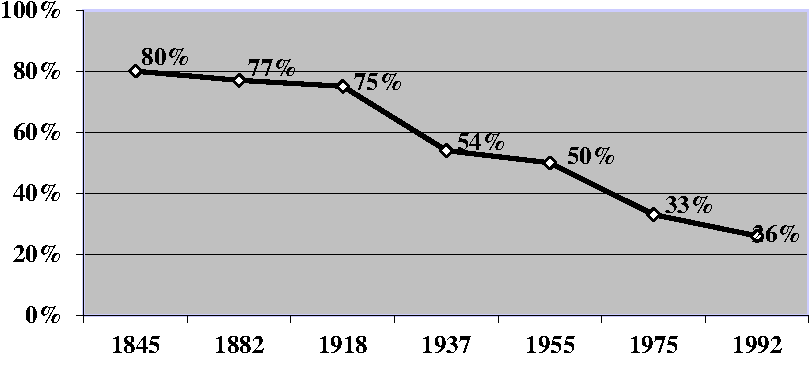
\includegraphics[width=.75\textwidth]{./img/fig1.pdf}
\caption{Null subjects in \gls{BP}\il{Brazilian Portuguese} in two centuries
(From \citealt{Duarte1993})}
\label{fig:key:26.1}
\end{figure}

The rates of null subjects across the periods analysed suggest three stages in
the process of change, which coincide with changes in the inflectional paradigm
triggered by apocope in the second person singular, a very common phenomenon,
and third person plural, a socially constrained phenomenon, as well as by two
important changes in the set of nominative\is{nominative case} pronouns, shown in
\Cref{tab:key:26.1}.\footnote{Considering that the first author was born in
    1815 and the fourth, in 1884, we could assume that the change took place in
    the turn of the Century. We are aware of the fact that tracing linguistic
    change over long periods of time implies using documents that do not
    capture the vernacular of their writers. Quoting
    \parencite[11]{Labov1994}, “historical linguistics can then be thought of
    as the art of making the best use of bad data”.}

\begin{table}[htpb]
    \centering
    \begin{tabularx}{1\textwidth}{lXXXX}
    \lsptoprule
                                             & Nominative\newline pronouns                   & Paradigm 1\newline19th century       & Paradigm 1\newline 20th century/1          & Paradigm 3\newline 20th century/2\\
    \midrule
    \Fsg{}                                   & eu                                            & cant\emph{o}                         & cant\emph{o}                               & cant\emph{o} \\
    \Ssg{}                                   & tu\newline \emph{você}                        & canta\emph{s}\newline ---            &
    canta\emph{s}\newline canta$\varnothing$ & canta(\emph{s})\newline canta$\varnothing$ \\
    \Tsg{}                                   & ele, ela                                      & canta$\varnothing$                   & canta$\varnothing$                         & canta$\varnothing$ \\
    \Fpl{}                                   & nós\newline \emph{a gente}                    & canto\emph{mos}\newline ---          & canta\emph{mos}\newline canta$\varnothing$ & canta\emph{mos}\newline canta$\varnothing$\\
    \Spl{}                                   & vós\newline \emph{vocês}
                                             & canta\emph{is}\newline canta\emph{m} & ---\newline canta\emph{m}                  & ---\newline canta(\emph{m}) \\
    \Tpl{}                                   & eles, elas                                    & canta\emph{m}                        & canta\emph{m}                              & canta(\emph{m}) \\
    \lspbottomrule
    \end{tabularx}
    \caption{Evolution of verbal inflectional paradigm in \gls{BP} ---
    \emph{cantar} \enquote*{to sing} (adapted
from~\citealt{Duarte1993})}\label{tab:key:26.1}
\end{table}

The plays written in the first three synchronies, exhibit six  and sometimes
five different forms, with a syncretism, represented by the address forms
\emph{o(a) senhor(a)} \enquote*{the lord}, \enquote*{the lady} and \emph{Vossa
Mercê} \enquote*{Your Grace}, which all combine with third person unmarked form
for singular.  This is what we attest for European Portuguese. The reduction of
null subjects in the 1930s and the 1950s is triggered by the
\isi{grammaticalization}
of \emph{Vossa Mercê} as \emph{você}, which is fully inserted in the pronominal
system as second person reference, while the pronoun \emph{tu} is abandoned by
some authors.\footnote{For some reason to be investigated, the most popular
    authors of this type of “light” plays written in Rio de Janeiro made an option
in favor of \emph{você}. The city population has not abandoned the use of
\emph{tu} but it was more restricted to the suburban areas, with a number of
new textile industries, where people born in the city were concentrated.} Those
who insist in keeping \emph{tu} and \emph{você} in the paradigm usually mix
both forms to address the same person, not only in nominative\is{nominative case} function but in
accusative and dative\is{dative case} functions as well.\footnote{This is real evidence of the
    \isi{grammaticalization} of \emph{você}; the loss of courtesy, originally
    distinguishing \emph{você}, is kept in European Portuguese, which maintains
    the complementary distribution between \emph{tu}, for family and close
    friends, and \emph{você}, usually null, for other social relations.
    Explicit \emph{você} coming from a stranger is not well accepted by older
Portuguese. See \citet{LopesBrocardo2016} with respect to current
\isi{grammaticalization} processes in \gls{BP}\il{Brazilian Portuguese}.} This change
was further aggravated by the entry of \emph{a gente} (the folks, the people,
similar in meaning to \ili{French} \enquote*{on}), in Paradigm 3, replacing
first person plural \emph{nós} (we), also requiring the unmarked third person
singular agreement, due to its nominal origin.

We have enough evidence from diachronic research, according to which both
processes started before the 19th century. With respect to \emph{a gente},
\citet{Lopes2003} shows that after a transitory period of ambiguity between a
nominal reading or its interpretation as a pronoun, it is in the end of the
19th Century that its full implementation is attested in variation with the
conservative pronoun \emph{nós} (we), which has an exclusive ending
\tuple{\text{-mos}}.  With respect to \emph{você} (you), \citet{Lopes2003}
claims that its variation with \emph{tu} (you) in letters, very sporadic in the
19th Century, enters the system slowly in the 20th Century. A side  effect of
this pronominalization is attested in the mixture of oblique and possessive
pronouns of second and third persons in letters and plays written from the
1930s on. Today, \emph{você} (in variation with \emph{tu}) and \emph{a gente}
are preferred not only for definite reference but for generic reference as
well, in which case the former may or may not include the speaker and the
addressee, the latter must include the speaker.

Such changes have been the most significant trigger for the “impoverishment” of
BP’s paradigm. Differently from the variable use of \tuple{\text{-s}} and \tuple{\text{-m}}, related to a
phonological process (apocope) and constrained by social factors, there is no
variation in the use of the unmarked verb form with the new pronouns derived
from DPs. The consequence was the loss of the \emph{functional richness}
of the inflectional paradigm, in \citegen{Roberts1993} terms. For
\citet{Galves1993}, this reduction entails the loss of the semantic feature in
the category \emph{person.} Associated with the feature \emph{number}, the
paradigm was reduced to four possible combinations:

\ea%5
    \label{ex:key:26.5}\leavevmode\\[-1\baselineskip]%
    \begin{tabular}{lllll}
    $+$person & / & $-$plural & $>$ & \emph{-o} \\
    $+$person & / & $+$plural & $>$ & \emph{-mos} \\
    $-$person & / & $+$plural & $>$ & \emph{-m} \\
    $-$person & / & $-$plural & $>$ & \emph{-}$\varnothing$ \\
    \end{tabular}
\z

Such an \emph{impoverished} or \emph{weakened} paradigm would certainly affect
the identification of an empty category.

The empirical evidence of the late implementation of the two new pronouns does
not sustain the claim that it could actually be the case that the set of
pronouns changed as a consequence of the changes in the inflectional paradigm.
The cases of apocope shown in the chart above were certainly a consequence of
contact. However, additional evidence that African slaves and their descendants
did not reduce the verbal paradigm drastically comes from important written
documents produced by Africans, who learned Portuguese as a second language in
the State of Bahia. Such documents, written in the 19th
Century – along the decades of 1830 and 1840 – consist of 53 Acts of the
\emph{Sociedade} \emph{Protetora} \emph{dos} \emph{Desvalidos} (Protecting
Society of the Helpless), a fraternity founded by Africans to protect one
another, which kept minutes (memoranda) of their regular meetings, written by
five members. \citet{AlmeidaCarneiro2009} analysed the expression of pronominal
subjects and their results show the preference for null subjects with rates of
68\% for \Fsg{}, 89\% \Fpl{}, 89\% for \Tsg{}, and 93\% for \Tpl{}. The
paradigm used in the memoranda includes the pronoun \emph{nós} for \Fpl{}
reference, with the canonical inflection \tuple{\text{-mos}}. The cases of non-agreement are
restricted to the apocope of \Tpl{} inflection \tuple{\text{-m}}. This discursive tradition
does not favour the use of second person. All the constraints pointed out as
favoring null subjects, such as co-reference and non-animate antecedents, are
confirmed. The only oscillation attested in the data is related to individual
performances – only one of the five authors shows a low rate of null subjects
(33\%); the other four exhibit overall rates above 77\%.

The analyses of spoken Portuguese acquired by  African descendants are not
different from those obtained by Brazilians. \citegen{Lucchesi2009b} analysis
of the expression of subjects based on the vernacular speech of four isolated
rural Afro-Brazilian communities in the state of Bahia, with different
historical and socio-economic backgrounds, shows the same rates attested by
\citet{Duarte1995} for contemporary Portuguese spoken in the city of Rio de
Janeiro.

Returning to the results in \Cref{fig:key:26.1}, Duarte shows that the course
of change is different with respect to first and  second person on one hand and
to third person on the other. In the last quarter of the 20th century null
first and second person subjects reach a means of 20\%. Third person, thanks to
the interaction of [+human] and [−human/-animate] referents, exhibits a slow
descendant curve (see \citealt{CyrinoEtAl2000}). Such results would be
confirmed by \citegen{Duarte1995} analysis of spoken Rio de Janeiro variety.
Referential pronominal subjects in root clauses are preferentially overt
\parencite{Duarte1995}.\footnote{In short answers we can have an apparent NS
    with third person, but we analyse this sort of structure as resulting from
the fronting/focalization\is{focalisation} of the inflected verb eventually accompanied by its
adjuncts, followed by the remnant \isi{movement} of the TP (cf.\
\citealt{Kato2016}).} Second person singular, which triggered and led the
change, reveals 10\% of null subjects, usually pragmatically identified
(\ref{ex:key:26.6}a); first person singular null subjects reach 25\%,
particularly when preceded by a functional category, such as a NegP, and AspP
(\ref{ex:key:26.6}b):

\ea\label{ex:key:26.6}\ili{Brazilian Portuguese}
    \ea
    \gll	$\varnothing$\tss{\Ssg} sabe {o que} é pinho de riga?\\
            {} know what is pine of riga\\
	\glt	‘Do you know what riga pine is?’
    \ex
	\gll	$\varnothing$\tss{\Fsg} não gosto de boxe.\\
            {} not like    of boxing\\
	\glt	‘I don´t like boxing’
    \z
\z

Third person subjects, as mentioned, are constrained by \isi{animacy} and structural
patterns. In root clauses \citet{Duarte1995} attested 36\% of null subjects,
usually identified by an antecedent bearing the same function in the adjacent
clause or by an antecedent with discursive prominence (cf.\
\citealt{BarbosaDuarteKato2005,KatoDuarte2014b}):

\ea%7
    \label{ex:key:26.7}\ili{Brazilian Portuguese}
    \ea
	\gll	Ela\tss{i} gosta de cozinhar. $\varnothing$\tss{\Tsg\tss{i}} Aprende com as amigas.\\
    she likes of to.cook.      {}    learns    with the friends.\\
	\glt	\enquote*{She likes to cook. She learns with her friends}
    \ex
	\gll	[ O meu irmão ]\tss{i}? $\varnothing$\tss{\Tsg\tss{i}}  Mudou pros Estados Unidos.\\
    {} the my brother?  {} {}     moved to.the United States.\\
	\glt	\enquote*{My brother? He's moved to the United States}
    \z
\z

In embedded clauses, co-reference still plays an important role
(\citealt{Modesto2000,FigueiredoSilva2000,DuarteSoaresdaSilva2016}, a.o.), with
a regular distribution between overt and null subjects. \citegen{Duarte1995}
data show 32\% of null subjects in this \isi{control} pattern with [+human] and 44\%
with [-animate] referents:\newpage

\ea%8
    \label{ex:key:26.8}\ili{Brazilian Portuguese}
    \ea
	\gll	mas \textbf{ele}\textbf{\tss{i}}  sentiu [ que
    $\varnothing$\tss{\Tsg\tss{i}}  era  o    único novo    ali,
    recém-casado \dots{}]\\
            but  he\tss{i}  felt   {} that {} was the only   young there, newly-married \\
	\glt	\enquote*{But he felt he was the only young guy there, newly married….}
    \ex
	\gll	{}[ \textbf{Esse} \textbf{filme} ]\tss{i} emocionou muita  gente   quando (ele)\tss{i} ficou pronto\\
            {} That film\tss{i} {} touched many  people  when \hphantom{(}he  was ready\\
	\glt	\enquote*{That film touched many  people when it was shown}
    \z
\z

A null subject in a subordinate clause without co-reference with the subject of
the main clause is still attested if the verb of the main clause has an
epistemic verb. In such contexts, which have the antecedent in an A’-position,
overt subjects are also far more frequent: (\citealt{MoreiradaSilva1983};
\citealt{FigueiredoSilva1996,FigueiredoSilva2000}, a.o.):

\ea\label{ex:key:26.9}\ili{Brazilian Portuguese}\\
    \gll	{}[ \textbf{O} \textbf{armazém} ]\tss{i} (\dots{}) {quer dizer,} \underline{acho} [ que $\varnothing$\tss{\Tsg\tss{i}} já é extinto ] né? ]\\
    {} the grocery-store {} {} {I mean} think.\Fsg{} {} that {}  already is extinct, {} see?\\
    \glt	\enquote*{The grocery store\dots{} I think it's now extinct}
\z

One significant difference between \ili{French} and Brazilian Portuguese noted
by \citet{Duarte1995} was the fact that, although the two \ili{Romance} languages
have lost null referential subjects, \ili{French} also lost the null expletive\is{expletives}
with the development of the expletives \emph{ce}  and \emph{il} while
\gls{BP}\il{Brazilian Portuguese} retained it:

\ea%11
    \label{ex:key:26.11}
    \ea \ili{French}\\
    \gll    Il fait froid.\\
            it is  cold\\
    \ex \ili{Brazilian Portuguese}\\
    \gll    \textbf{$\varnothing$}\tss{\Expl} Faz frio./ $\varnothing$\tss{\Expl} Está frio.\\
            {} does cold {} is cold\\
    \z
\z

\ea%12
    \label{ex:key:26.12}
    \ea \ili{French} (apud \citealt[151]{Roberts1993})\\
    \gll    {\textbf{Il} i} avoit bien .xxiiij.M.   archiers {a piet}\\
            there were about 24.000 archers marching\\
    \newpage
    \ex \ili{Brazilian Portuguese}\\
    \gll    $\varnothing$\tss{\Expl} havia {bem uns} 24.000    arqueiros {a pé}\\
            {}  was about 24.000 archers marching\\
    \z
\z

With the loss of the generic clitic \emph{se}, BP shows a NS in
generic constructions,\footnote{Since the arbitrary clitic \emph{se} is also
    extinct in speech, \gls{BP} also exhibits a null arbitrary subject
    \parencite{Rodrigues2004}, in very modest rates, attested in variation
with the use of a 3rd person plural verb with a null or an overt pronoun
\emph{eles} (they).} while \ili{French} has the indefinite pronoun \emph{on}.

\ea%13
    \label{ex:key:26.13}
    \ea \ili{French}\\
        \textbf{On} ne voit plus de rémouleurs.
    \ex \ili{Brazilian Portuguese}\\
        $\varnothing$ Não vê mais amolador-de-faca.\\
        ‘One doesn’t see knife sharpeners any more.’
    \z
\z

However, in both languages, these constructions have nominative\is{nominative case} pronouns as
variants, largely preferred in \gls{BP}:

\ea\label{ex:key:26.14}
    \ea \ili{French}\\
        Vous / On ne voyez  plus de rémouleurs. Nous ne voyons plus de rémouleurs.
    \ex\ili{Brazilian Portuguese}\\
        Você / A gente não vê  mais amolador-de-faca\\
        ‘You / we don't see knife sharpeners anymore.’
    \z
\z

There are even contexts, as illustrated in \eqref{ex:key:26.15}, where a null
generic is ungrammatical in \gls{BP}\il{Brazilian Portuguese}:

\ea%15
    \label{ex:key:26.15}\ili{Brazilian Portuguese}\\
    \gll	Quando \textbf{a} \textbf{gente} / \textbf{você} / *$\varnothing$\textbf{\tss{\Genc}} é  menor, \textbf{a} \textbf{gente} / \textbf{você} não dá muito valor a essas coisas.\\
            when the people {} you {} {} are little, the people {} you not  give much value to these things\\
	\glt	\enquote*{When we /you are young, we / you do not value such things}
\z

Summarizing, our empirical analysis reveals that null referential subjects are
much less frequent than overt pronominals. Furthermore, the null generic
subject is not the most productive strategy to represent this type of
indeterminate subject; in addition, recent research does not show any sign of
increasing use of it among younger generations (see~\citealt{MarinsEtAlta}).
This might support the hypothesis that null subjects in \gls{BP}\il{Brazilian
Portuguese} could be residual cases still reflecting the replaced null subject
system, as far as referential (definite and indeterminate --- either arbitrary
or generic) uses are concerned. We will return to this matter in the following
section.

\section{Core grammar and I-language}\label{sec:key:26.2.3}

The theory of \glsunset{UG}\gls{UG}\is{Universal Grammar} tries to account for the acquisition\is{language acquisition} of
\emph{core} grammars through parameter\is{parameters} setting in a context of poverty of
stimulus \citep{Chomsky1986}, which can be understood partly as data containing
competing forms due to different values of the same parameter\is{parameters} coexisting in the
input that children receive. This is exactly the situation that a child faces
when there is a recent change or a change in progress as shown by the
well-studied case of the Null Subject (NS) in Brazilian Portuguese (BP).

As we saw above, in the \isi{I-language} of most literate Brazilian adults, a range
of referential NSs are possible, competing with the innovative pronominal
subjects. It is the case of the optionality of NSs and pronouns in complement
clauses as in example \REF{ex:key:15/2}:

\ea%15
    \label{ex:key:15/2}\ili{Brazilian Portuguese}\\
	\gll	O Pedr\textbf{o}\tss{i} disse que (\textbf{ele}\tss{i}) fala bem     espanhol.\\
            the Peter said that \hphantom{(}he speaks well  Spanish\\
	\glt	\enquote*{Peter said that  he speaks Spanish well.}
\z

Assuming, with \citet{Kato2011},\footnote{See also \citeauthor{Dresher1999}'s
(\citeyear{Dresher1999}, a.o.) theory according to which children do not reset
parameters.\is{parameters}} that \emph{core} grammars do not admit morphological “doublets”,
and that children have only the innovative variant, we will see that pre-school
children do not have pronouns competing with referential null subjects as in
the above context. \citeauthor{Kato2011} borrows data from
\textcite{Magalhaes2003}, who argues that referential NSs in
\gls{BP}\il{Brazilian Portuguese} are learned in school, where old forms are
provided through instruction.\largerpage[1]

\begin{table}[htpb]
    \centering
    \begin{tabularx}{\textwidth}{lXXX}
    \lsptoprule
                         & Pre-school & 3rd/4th grades & 7th/8th grades\\
    \midrule
    Pronominal subjects & 97.89\%    & 78.0\%         & 50.38\%\\
    Null subjects       & 2.11\%     & 22.0\%         & 49.62\%\\
    \lspbottomrule
    \end{tabularx}
    \caption{Pronominal and null subjects in complement clauses (adapted
    from~\citealt{Magalhaes2003})}\label{tab:key:26.2}
\end{table}

When the child masters complex clauses in pre-school, the NS is still almost
inexistent in his/her oral production of complement clauses. NSs start to
increase very quickly in their written performance, achieving the status of an
equal variant of the overt pronoun at the end of 8th
grade.\footnote{\citet{KatoEtAl2009} arrive at a similar conclusion
    with regard to Null Objects,\is{null objects} but in the opposite direction. Children have
    only Null Objects\is{null objects} in their \isi{core grammar}, and acquire the lost 3rd person
clitic at school.}

Several studies try to analyse the nature of the NS in such constructions,
where optionality is found in the adult’s \isi{E-language}, but what we are actually
studying is a variant learned at school, and one may ask whether these NSs are
an object of \gls{UG}. We will return to this problem in the following
sections.

The conclusion is that the only type of null subject licensed in
\gls{BP}\il{Brazilian Portuguese} \emph{core} grammar are the non-referential
NSs, namely the null expletive\is{expletives} and the generic subjects without the clitic
\emph{se}, as they are attested during language acquisition\is{language acquisition}.

\ea%16
    \label{ex:key:26.16}\ili{Brazilian Portuguese}
    \ea \textcite{Simoes2000}\\
    \gll    $\varnothing$\tss{\Expl} Tem dois aviões aqui.\\
            {} there-are two planes here.\\
    \ex \textcite{Magalhaes2007}\\
    \gll    $\varnothing$\tss{\Genc} pode chupar o dedo?\\
            {} can  suck the finger\\
    \z
\z

As for the \isi{E-language} exhibited by the literate adult, it will be shown that
the non-referential null subjects are the same as those of the Brazilian child,
but the null referential ones are in variation with the overt pronominal ones.

\section{Comparing the NS in BP with different types of
languages}\label{sec:key:26.3}

\subsection{BP vs.\ EP, a consistent NS language}\label{sec:key:26.3.1}

\citet{CarSta1994} distinguish three types of pronouns: strong, weak and
clitic.  Following \citet{Kato1999} we will make an initial split between
strong and weak forms, and will assume that weak pronominals can be one of
three types: i) free pronouns, like in \ili{English}, ii) \isi{clitics} as in
Trentino, a Northern \ili{Italian} dialect or iii) agreement affixes, or
pronominal Agr as in \ili{Italian} and \gls{EP}\il{European Portuguese} (cf.\
Fig 2). The weak pronominals are Agreement affixes in the so-called consistent
\emph{pro-drop} languages. All languages, on the other hand, dispose of strong
pronouns, which exhibit a “default” case
(\citealt{Kato2000,Schutze2001}).\footnote{Moreover, strong pronouns are always
deictic, or referential, while weak pronouns can be deictic or referentially
dependent.  Strong pronouns are always [+human] while weak pronouns can be
[+human] or [−human].}

\ea\label{tree:fig2}
    
\begin{tikzpicture}[baseline=(root.base), align=left]

        \Tree 	[.\node(root){Pronouns};
                    [.Strong
                        {English\\Trentino}
                    ]
                    [.Weak
                        {Free\\English}
                        {Clitics\\Trentino}
                        {Pronominal Agr\\Italian}
                    ]
                ]

    \end{tikzpicture}
\z

\citegen{Salvi1997} conclusions on what happened in the beginning of \ili{Romance}
seem to partially support what is being proposed here. Studying the changes
from \ili{Latin} to Old \ili{Romance} and from Old \ili{Romance} to \ili{French} and the Northern
\ili{Italian} dialects, he concludes that: (a) \ili{Latin} had only one form of
nominative pronouns, which, he assumes, were used as strong or weak pronouns,
b) in Old \ili{Romance} pronominal anaphora was not obligatory since subject \isi{clitics}
did not exist; (c) in \ili{French} and in some \ili{Italian} dialects zero
anaphora  (NS) ceases to exist when subject \isi{clitics} appear (see also
\citealt{Roberts1993}).

For \citet{Kato1999},\footnote{See also similar views in
\citet{Barbosa1995,AleAna1998,OrdonezTrevino1999}.} pronominal Agr, understood
as the \isi{grammaticalization} / incorporation of personal pronouns in verbal
Inflection, is claimed to be in crosslinguistic complementary distribution with
weak pronouns and subject \isi{clitics}. Thus, the loss of one implies the
introduction of the other type of weak pronouns.\footnote{Studying the loss of
    NSs in \ili{Dominican Spanish} and
\gls{BP}\il{Brazilian Portuguese}, \textcite[28]{Camacho2016} proposes, in
line with \citet{Kato1999}, that the change has to do with “modification in the
lexical entries for inflection”, namely the introduction of weak pronouns.}

In \gls{BP}\il{Brazilian Portuguese} the great innovation was the introduction
of an English-like paradigm of weak pronouns partially homophonous with the
strong ones \parencite{Nunes1990,Kato1999} in place of the old pronominal Agr
system.\footnote{In written language the new paradigm is represented as
homophonous to the strong pronouns.}

\ea\label{ex:key:26.17}\leavevmode\\[-1\baselineskip]
    \begin{tabular}{llll}
    Strong     & weak     & Strong      & weak \\
    EU (I)     & [eu/ô]   & NÓS (we)    & [nós] \\
    VOCÊ (you) & [cê      & VOCÊS (you) & [cêis] \\
    ELE (he)   & [ele/ei] & ELES (they) & [eles/eis] \\
    \end{tabular}
\z

Pronominal Agr is syntactically defined by \citet{Kato1999} as a D-category
that appears in the numeration as an independent item from the verb, being
first merged as an external argument of \emph{v}, with interpretable
φ-features\footnote{\citegen{Kato1999} analysis above eliminated \emph{pro},
    and its problems in a Minimalist frame: (a) the position of \emph{pro}
    ceases to be a problem, (b) its presence in the numeration is eliminated and
    (c) it will give a coherent explanation on why there is free inversion since
it will be moving a maximal projection. Brazilian Portuguese, on the other
hand, cannot move T’, the reason why it lost free inversion.}.  There is no
Spec of T/INFL projected, as the pronominal agreement satisfies the
\glsunset{EPP}\gls{EPP} morphologically. In \gls{BP}\il{Brazilian Portuguese}
with Agr no longer pronominal, free weak pronouns are introduced, and Spec of
T/INFL has to be projected. In \gls{EP}\il{European Portuguese}, on the other
hand, pronominal Agr remained and, therefore, no weak free pronouns were
created.

\begin{exe}
\ex Pronominal Agr and weak pronouns\label{ex:key:26.fig3}\\
\noindent\begin{minipage}[t]{.5\textwidth}
    \sn
    \begin{xlist}
    \exi{a.} Before the change (\gls{EP})\\
    
\begin{tikzpicture}[baseline=(root.base)]

        \Tree 	[.\node(root){TP};
                    [.T
                        -o\tss{i}
                        fala-V
                    ]
                    [.VP
                        [.DP [.D t\tss{i} ] ]
                        [.V$'$ [.V t\tss{V} ] ]
                    ]
                ]

    \end{tikzpicture}
    \end{xlist}
\end{minipage}
\noindent\begin{minipage}[t]{.5\textwidth}
    \sn
    \begin{xlist}
    \exi{b.} After the change (\gls{BP})\\
    
\begin{tikzpicture}[baseline=(root.base)]

        \Tree 	[.\node(root){TP};
                    [.DP eu ]
                    [.T$'$
                        [.T falo-V ]
                        [.VP
                            [.DP t\tss{i} ]
                            [.V t\tss{V} ]
                        ]
                    ]
                ]

    \end{tikzpicture}
    \end{xlist}
\end{minipage}
\end{exe}

Strong pronouns are in a higher projection than weak pronouns. This higher
projection can be ΣP, as in \citet{Martins1994}, or the SubjP in
\citet{Cardinaletti:2004a}. When the pronoun is overt in \gls{NSL}s, it always
has an emphatic or contrastive interpretation. If a non-NS language has an
overt pronoun, the sentence exhibits subject doubling, as in
\gls{BP}\il{Brazilian Portuguese} (cf.\ examples \eqref{ex:key:26.18}, apud
\citealt{Kato2012}). But in either case, strong pronouns have a “default” case
and are always referential and  [+animate] (\citealt{Kato1999},
\citealt{Schutze2001}).\newpage

\begin{exe}
\ex Position of strong pronouns\label{ex:key:26.fig4}\\
\noindent\begin{minipage}[t]{.5\textwidth}
    \sn
    \begin{xlist}
    \exi{a.} Before the change (\gls{EP})\\
    \hspace*{-1.0cm}\begin{tikzpicture}[baseline=(root.base), align=center,
        scale=.9]

        \Tree 	[.\node(root){ΣP/SUBJP};
                    [.DP VOCÊ ]
                    [.{}
                        Σ
                        [.TP
                            [.T
                                -$\varnothing$\tss{i}
                                come-\tss{V}
                            ]
                            [.VP
                                [.DP {D\\t\tss{i}} ]
                                [.V$'$
                                    {V\\t\tss{V}}
                                    {DP\\pizza}
                                ]
                            ]
                        ]
                    ]
                ]

    \end{tikzpicture}
    \end{xlist}
\end{minipage}
\noindent\begin{minipage}[t]{.5\textwidth}
    \sn
    \begin{xlist}
    \exi{b.} After the change (\gls{BP})\\
    \hspace*{-1.5cm}\begin{tikzpicture}[baseline=(root.base), align=center,
        scale=.9]

        \Tree 	[.\node(root){ΣP/SubjP};
                    [.DP VOCÊ ]
                    [.{}
                        Σ
                        [.TP
                            [.DP cê ]
                            [.T$'$
                                [.T come-\tss{V} ]
                                [.VP
                                    [.DP t\tss{i} ]
                                    [.V$'$
                                        {V\\t\tss{V}}
                                        {DP\\pizza}
                                    ]
                                ]
                            ]
                        ]
                    ]
                ]

    \end{tikzpicture}
    \end{xlist}
\end{minipage}
\end{exe}

\ea%18
    \label{ex:key:26.18}
    \ea \ili{European Portuguese}\\
    \gll    VOCÊ,   come-${\varnothing}$ pizza.\\
            you      eat      pizza\\
    \ex \ili{Brazilian Portuguese}\\
	\gll	VOCÊ,   cê    come pizza\\
			YOU    you  eat pizza\\
	\glt	\enquote*{YOU, you eat pizza.}
    \z
\z

Taking into consideration that the referential NS of the literate Brazilian
adult has been acquired through schooling, we can bring some interesting
results from \citeauthor{BarbosaDuarteKato2005}’s study as to what extent
instruction recovers the “\isi{Avoid Pronoun Principle}”, which seems to rule the
speakers of a consistent \gls{NSL}\is{null subject languages}.
\Cref{fig:key:26.2} shows null subjects in spoken \gls{EP}\il{European
Portuguese} and \gls{BP}\il{Brazilian Portuguese}.\largerpage[-2]

\begin{figure}[htpb]
    \centering
    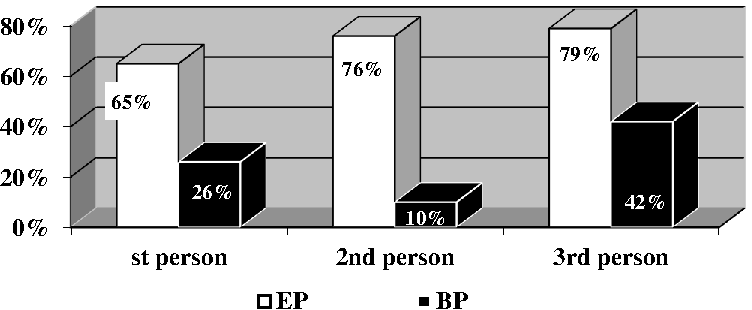
\includegraphics[width=0.75\linewidth]{./img/fig2.pdf}
    \caption{Null subjects in spoken \gls{EP} and \gls{BP} (adapted
    from~\citealt{BarbosaDuarteKato2005}, Figure 3,
apud~\citealt{Duarte2004})}\label{fig:key:26.2}
\end{figure}

Despite the fact that schools in Brazil try to
provide the students with the old NS grammar, Brazilians produce a much higher
proportion of overt pronouns than Portuguese speakers, following the same
hierarchy (see examples \eqref{ex:key:26.6} to \eqref{ex:key:26.9} in
\Cref{sec:key:26.2.2}.). As we mentioned in \Cref{sec:key:26.2.2}, this has
been related to (a) the neutralization of \emph{tu} and \emph{você} (second PS)
for second person reference. (b) the replacement of \emph{vós} by \emph{vocês}
(second PP), and (c) the introduction of \emph{a} \emph{gente}  in competition
with \emph{nós}, which reduced the inflectional paradigm (See
\tabref{tab:key:26.1}), requiring the overt pronoun for identification
reasons.\footnote{Most regions of the country that keep the pronoun \emph{tu},
    combine it, in colloquial speech, with the same unmarked third person verb
    form used with \emph{você} (\emph{tu}/\emph{você} \emph{fala} – you speak).
    Evidence for the neutralization of both pronouns is in the fact that they
    are used without any distinction as regards courtesy, contrary to what
happens in Portugal.}

As for qualitative distinctions \citeauthor{BarbosaDuarteKato2005}
(\citeyear[19]{BarbosaDuarteKato2005}, BDK) listed the following observations:

\paragraph*{(a)} A significant difference between the two varieties is in the
fact that overt pronouns in \gls{EP}\il{European Portuguese} are almost
invariably [+animate], which shows that they are generally strong pronouns,
while in \gls{BP}\il{Brazilian Portuguese} they can be [+animate] or
[-animate], indicating that they can be strong or weak.

\ea\label{ex:key:26.19}
    \ea\ili{European Portuguese}\\
	\gll	Os miúdos  vão pra     escola e     ela vai    pro      escritório.\\
			the children go    to.the school and she goes to.the   office\\
	\glt	\enquote*{The children go to      school and she goes to the office.}
    \ex\ili{Brazilian Portuguese}\\
	\gll	Eu acho que um trabalho\tss{i}, ele\tss{i} teria  que começar por aí.\\
			I think   that a   task           it should-have to start       from there.\\
	\glt	\enquote*{I think that  a task should have to start from here.}
    \z
\z

\paragraph*{(b)} The \isi{control} relation between the antecedent and the null
subject is the most favourable context for NSs in both varieties, even though
\gls{BP}\il{Brazilian Portuguese} prefers overt subjects; in
\gls{EP}\il{European Portuguese}, on the other hand, a null subject is
categorical, as in (\ref{ex:key:26.20}), the exceptional cases having to do with
emphatic/contrastive strong ones.

\ea%20
    \label{ex:key:26.20}\ili{European Portuguese}\\
	\gll	Ela\tss{i} disse logo que \textbf{$\varnothing$}\tss{i} tava em
    férias e que \textbf{$\varnothing$}\tss{i} morava ali {ao pé} do liceu.\\
            she said soon that {} was on vacation  and  that {} lived there
            near of.the liceum\\
	\glt	\enquote*{She soon said that she was on vacation and that she lived there near the school.}
\z

\paragraph*{(c)} The real variation domain of null and expressed subjects in
both varieties is where no \isi{control} relation obtains. It seems to be correlated
with a functional factor, namely topic maintenance, which favours the NS, vs
topic shift, favouring overt pronouns. (cf.\ also \citealt{DeOliveira2000} and
\citealt{Marins2009} with respect to Italian). However, a consistent NSL will
prefer a null subject even in anaphoric contexts.

\ea%21
    \label{ex:key:26.21}\ili{European Portuguese}
    \ea
	\gll	Quando eu estava a trabalhar com ele\tss{i} \textbf{$\varnothing$}\tss{i} nunca me     queria ver na cozinha\\
            when     I   was     at work       with he {} never  me.\Cl{} wanted to.see in.the kitchen\\
	\glt	\enquote*{When I was at work with him, he never wanted to see me in the kitchen.}
    \ex
	\gll	Parece que numa ida d[ela]\tss{i}     à   Inglaterra, ela\tss{i} fez     com que   a rainha pedisse nossos produtos.\\
			seems   that in.a   trip of.her to.the England,    she made with that  the queen ordered our products\\
	\glt	\enquote*{It seems that in one of her trips to England she made the queen order our products.}
    \z
\z

To account for the finding that \gls{BP}\il{Brazilian Portuguese} still
licenses NSs, as opposed to a language like \ili{English}, we have had two
lines of explanation:

\paragraph*{(a)} they result from the fact that we have a change in progress,
with two grammars in competition (\citealt{Duarte1993,Duarte1995};
\citealt{Kato2000}), the NSs being residual occurrences of the  same NS of the
old grammar;

\paragraph*{(b)} the NS in \gls{BP}\il{Brazilian Portuguese} is not a
pronominal Agr,  but (b1) a variable bound by a quantifier
\parencite{NegraoMuller1996}; (b2) a variable or an anaphor
\parencite{FigueiredoSilva2000}; (b3) a variable bound by a Topic, the subject
in \gls{BP}\il{Brazilian Portuguese} being in A’-position \citep{Modesto2000};
(b4) the trace of A-movement
\parencite{Ferreira2004,Rodrigues2004,MartinsNunes2009}.

However, according to the data in \textcite{BarbosaDuarteKato2005} and in
\citet{Kato2009}, the theories in (b) do not explain the optionality in real
data, namely the presence of overt pronouns, where the NS would be the only
option.

\ea\label{ex:key:26.22}\ili{Brazilian Portuguese}
    \ea \textcite{NegraoMuller1996}\\
    \gll    \textbf{Nenhuma} \textbf{criança} acha que \textbf{$\varnothing$}\tss{i} / *ela é burra.\\
            no child     thinks that {} {} \hphantom{(}she is stupid\\
    \ex \textcite{BarbosaDuarteKato2005}\\
    \gll    \textbf{Ninguém} \textbf{no} \textbf{Brasil}\tss{i} acha    que \textbf{ele}\textbf{\tss{i}} é prejudicado pelo governo.\\
            nobody    in Brazil   thinks  that he is  impaired     by-the government\\
    \z
\z

\ea%23
    \label{ex:key:26.23}\ili{Brazilian Portuguese}
    \ea     \textcite{FigueiredoSilva2000}\\
	\gll	A Maria achou um carro que *\textbf{$\varnothing$}\tss{i} tem grana pra comprar. \\
			the Maria  found   a   car     that  {} has money  to buy\\
	\glt	\enquote*{Mary found  a car that she has money to buy.}
    \ex     \textcite{Kato2009}\\
	\gll	A Maria\tss{i} achou o carro que \textbf{$\varnothing$}\tss{i} queria.\\
			the Maria    found  a car     that {} wanted\\
	\glt	\enquote*{Mary found a car that she wanted.}
    \z
\z

\ea%24
    \label{ex:key:26.24}\ili{Brazilian Portuguese}
    \ea     \textcite{Modesto2000}\\
	\gll	Paulo\tss{1} convenceu o Pedro\tss{2} que  \textbf{$\varnothing$}\tss{1/*2/*3} tinha que ir embora.\\
            Paulo  convinced the Pedro that {} had to go home\\
	\glt	\enquote*{Paulo convinced Peter that he had to go home.}\newpage
    \ex     \textcite{Kato2009}\\
    \gll	O Paulo\tss{1} convenceu \textbf{o} \textbf{Pedro}\textbf{\tss{2}} que \textbf{$\varnothing$}\textbf{\tss{1/2}} devia estudar mais.\\
			the Paulo convinced the Peter that {} should study more\\
	\glt	\enquote*{Paul convinced peter that he should study more.}
    \z
\z

Working with the \isi{raising} phenomenon in \gls{BP}\il{Brazilian Portuguese},
\citet{MartinsNunes2009} try to give an account of optionality seen in
\eqref{ex:key:26.25} below as a matter of acquisition\is{language acquisition}, in line with what we saw
in \Cref{sec:key:26.2.3}.  According to these authors, children start with the
parameter in \gls{BP}\il{Brazilian Portuguese} set as [-]NS, with only
(\ref{ex:key:26.25}a) as a possibility, but later, in view of the input of
literate speakers or writers, they add the possibility of an optional defective
T in their grammar, which is incapable of  checking  the features of a raised
subject.

\ea%25
    \label{ex:key:26.25}\ili{Brazilian Portuguese}
    \ea     \textcite{MartinsNunes2009}\\
	\gll	Os vizinhos    parecem    que compraram um carro.\\
            the neighbors seem.\Tpl{} that bought.\Tpl{}  a car\\
    \ex     \textcite{MartinsNunes2005}\\
	\gll	Os vizinhos, \textbf{$\varnothing$}\textbf{\tss{i}} parece     que t\tss{i} compraram um carro.\\
            the neighbors, {} seem.\Tsg{}    that {} bought        a car\\
	\glt	\enquote*{The neighbours seem to have bought a car.}

    \z
\z

As in \citet{MartinsNunes2009} and \citet{Kato2011}, the hypothesis that we
will be considering, is that the Brazilian child has set the \gls{NSP} to its
negative value, and that the referential NSs in \gls{BP}\il{Brazilian
Portuguese} adult data result from the imperfect learning of a “second
grammar”.

\subsection{BP vs.\ Japanese, a radical NS language}\label{sec:key:26.3.2}

A radical\is{null subject languages!radical null subject languages} null subject (NS) language has been defined as one without rich
agreement, like, for instance, Chinese and \ili{Japanese}, also referred
to as \emph{discourse configurational} (DC) languages
\parencite{EKiss1995,Miyagawa2010} or Topic-prominent languages
\parencite{LiThompson1976}.\footnote{The first author of the paper is a speaker
of Japanese as L1, and of \gls{BP}\il{Brazilian Portuguese} as L2, but more
fluent in the later.} Three reasons lead Brazilian linguists to hypothesize
that \gls{BP}\il{Brazilian Portuguese} is changing towards a DC type of
language\footnote{See the first  proposals in \citet{Pontes1987} and
    \citet{Kato1989}.  Actually they propose that \gls{BP}\il{Brazilian
Portuguese} is a Topic and Subject prominent language in
\citegen{LiThompson1976} terminology.   More recently, see
\citet{NegraoViotti2000,Modesto2008} with a similar view.}: (a)
\gls{BP}\il{Brazilian Portuguese} lost rich agreement,  (b) like other DC type
of language, \gls{BP}\il{Brazilian Portuguese} not only has NSs, but also Null
Objects and Bare Nouns, and (c) like other DC types of language,
\gls{BP}\il{Brazilian Portuguese} does not dispose of lexical expletives, in
accordance with \citegen{LiThompson1976} assumption for Topic prominent
languages.\footnote{\textcite{KatoDuarte2014a} proposed the \isi{movement} of an
    internal constituent to SpecTP in \gls{BP}, instead of the direct merging
    of the null expletive\is{expletives} (cf.\ \citealt{Chomsky2004}). But, in later work,
\textcite{KatoDuarte2014b} show that the two resulting constructions co-exist,
one in categorical constructions and the other in the thetic one.}

With existential sentences, what we have in Japanese, instead of the expletive\is{expletives},
is the morpheme  \emph{-ga} marking the subject. For the locative raised ones,
we have \emph{-wa}, the topic marker.  A sentence with \emph{-ga} is
interpreted as a thetic, or a presentational, sentence, while a sentence with
\emph{-wa} is interpreted as a categorical (or predicational) one\footnote{See
    \citet{Kuroda1972} for this terminology.  Existential sentences are typical
    thetic sentences. In \gls{BP}\il{Brazilian Portuguese} the subject is a
null expletive\is{expletives} when it is a thetic sentence, but if the locative raises to
subject position it is a categorical sentence like sentences with \emph{-wa} in
Japanese.}.

\ea%26
    \label{ex:key:26.26}\ili{Brazilian Portuguese}
    \ea
    \gll \textbf{$\varnothing$} Tem dois cachorros no quintal.\\
        has two dogs in.the yard\\
    \ex
    \gll (N)o quintal  tem dois cachorros.\\
        in.the yard has two dogs\\
    \glt \enquote*{There are two dogs in the yard.}
    \z
\z

\ea%27
    \label{ex:key:26.27}\ili{Japanese}
    \ea
    \gll    Inu-\textbf{ga} nihiki  niwa-ni iru.\\
            dog-\Nom{}  two yard-\Loc{} aru\\
    \ex
    \gll    Niwa-ni-\textbf{wa} inu-\textbf{ga} nihiki iru.\\
            yard-\Loc{}-\Topic{} dog-\Nom{} two are\\
    \z
\z

Weather constructions in \gls{BP}\il{Brazilian Portuguese} have (a) the verb
denoting the climatic event with a null expletive\is{expletives} as the subject  (cf.\
(\ref{ex:key:26.28}a), or  (b) like Japanese, the subject denoting  the event
with a general verb of motion \emph{cair} \enquote*{fall} as in
(\ref{ex:key:26.28}b).  The third possibility is locative \isi{raising} to the
subject position (\ref{ex:key:26.28}c).  Moreover, in this case the sentence is
categorical and the subject triggers agreement in \gls{BP}\il{Brazilian
Portuguese}, but not in Japanese.

\ea%28
    \label{ex:key:26.28}\ili{Brazilian Portuguese}
    \ea
	\gll	$\varnothing$ Está nevando  desde ontem nesta cidade.\\
			{} is  snowing    since yesterday in.this city\\
	\glt	\enquote*{It is snowing since yesterday in this city.}
    \ex
	\gll	A neve   cai   desde ontem   nesta cidade.\\
			the snow falls since yesterday in.this city\\
	\glt	\enquote*{The snow falls since yesterday in this city.}, \enquote*{The snow is falling since yesterday in this city.}
    \ex
	\gll	As cidades nessa região nevam muito.\\
            the cities    in.this region  rain.\Tpl{} {a lot}\\
	\glt	\enquote*{In the cities in this region it rains a lot.}
    \z
\z

\ea%29
    \label{ex:key:26.29}\ili{Japanese}
    \ea
	\gll	Yuki-\textbf{ga}   kinoo-kara         fute-iru.\\
            snow-\Nom{} yesterday-since  raining-is\\
	\glt	\enquote*{The snow falls since yesterday.}
    \ex
	\gll	Kono-hen-no matchi-\textbf{wa}  yoku yuki-\textbf{ga}      furu .\\
            {this region} city–\Topic{} well snow-\Nom{}  fall\\
	\glt	\enquote*{The cities in this region snow a lot.}
    \z
\z

But besides the existential and the weather verb sentences,
\gls{BP}\il{Brazilian Portuguese} has another NS similar to Japanese, namely
the null generic and arbitrary sentences.

\ea%30
    \label{ex:key:26.30}\ili{Brazilian Portuguese}
    \ea
	\gll	$\varnothing$ conserta sapato.\\
			{}  repairs shoes\\
    \ex
	\gll	$\varnothing$ kutsu-o       nao-shimasu.\\
            {}  shoes-\Acc{}   repair-do\\
	\glt	\enquote*{One repairs shoes.}
    \z
\z

In order to analyse the NS of generic and arbitrary sentences, \citet{Kato2000}
made use of PRO for finite contexts, adapting \citegen{Huang1989} idea of
\emph{generalized \isi{control} theory}.  We can support this view as, with the
deterioration of inflection, finite sentences tend to behave as infinitive or
gerundive clauses. Kato also assumes that PRO is the strong null third person
pronoun and we are assuming with \citet{Tomioka2003} that the weak pronoun in
Japanese is a Null Noun. We would have the following representation in
\gls{BP}\il{Brazilian Portuguese} for a non-referential generic sentence with
the NS.  The nominal [\tss{NP} $\varnothing$] in \eqref{ex:key:26.31} would
correspond to the \ili{English} nominal \emph{one}, or the \ili{French}
\emph{on.}

\ea%31
    \label{ex:key:26.31}
    {}[ PRO\tss{i} [ [\tss{NP} $\varnothing$]\tss{i} conserta sapato]
\z

Just like with existentials, we can have \isi{raising} of a locative, both in
\gls{BP}\il{Brazilian Portuguese}  and Japanese, with the same categorical
reading

\ea%36
    \label{ex:key:26.36bp}
    \ea\ili{Brazilian Portuguese}\\
        Aqui conserta sapato.
    \ex\ili{Japanese}\\
        Koko-de-\textbf{wa}  kutsu-o nao-su.\\
        ‘Here one repairs shoes.’
    \z
\z

This parallel behaviour between agreement and a Discourse feature can be
explained in terms of \citet{HolNik2002}, for whom Topic\is{topic} and
Focus\is{focus} are
formal features, equivalent to \isi{φ-features}. \citegen{Miyagawa2010} implements
this idea in an interesting way to derive Agreement languages vs Discourse
Configurational Languages.  In his analysis, discourse features forces \isi{movement}
in the same fashion as does agreement. In the spirit of
\citeauthor{Chomsky2007}’s (\citeyear{Chomsky2007,Chomsky2008})
proposal of merging \isi{φ-features} in C, with their subsequent percolation to
T,\footnote{Miyagawa uses φ-probes, instead of \isi{φ-features}.} Miyagawa’s proposal
is to merge the discourse-features (\isi{δ-features}) in C as an  alternative  to the
φ{}-features, which would also trigger
movement.\footnote{\textcite{NavesEtAl2013} provide the first attempt to analyse
    \gls{BP}\il{Brazilian Portuguese} using Miyagawa’s theory.  Though  it is
    similar in approach, the purpose of the present analysis  is to compare
Japanese and \gls{BP}\il{Brazilian Portuguese} using the same theoretical
frame.} He admits, moreover, that there are also mixed types of languages,
such as \ili{Turkish}, which can percolate both types of features.

We may say that \gls{BP}\il{Brazilian Portuguese} is this mixed kind of
language as \isi{raising} is triggered if the DP is a topic, but, at the same time, T
inherits agreement features, as can be seen in (\ref{ex:key:26.28}c).

\subsection{BP: A PNS language?}\label{sec:key:26.3.3}

This section brings some support to Biberauer’s comment, presented at the
beginning of this chapter, namely to the fact that this group seems
to include several sub-types of languages.

According to \citegen{HolNik2002} well-known article on Finnish, this language
has the following properties related to the subject position: (a) it has a rich
agreement system; (b) but, contrary to consistent \gls{NSL}s, the NS is
\emph{optional} (even though extremely rare in speech) with first and second
persons (36a,b) while third person subjects, animate or inanimate, must be
\emph{overt} in matrix clauses (\ref{ex:key:26.36}c), with null subjects
allowed only in embedded clauses under the requirement that they be bound by
the closest controller (see similar examples for \gls{BP}\il{Brazilian
Portuguese} in \eqref{ex:key:26.8} and \eqref{ex:key:26.9} in
\Cref{sec:key:26.2.2}); (c) expletives can be optional with weather-verbs and
extraposed sentences (\ref{ex:key:26.36}d); (d) but are obligatory with
existential type of predicates  (\ref{ex:key:26.36}e), and e) it is a topic
prominent language in the sense that the \gls{EPP} can be satisfied only by
referential categories, such as temporal adverbials and locatives or even DPs,
apparently to avoid V1 (\ref{ex:key:26.36}e), (\ref{ex:key:26.37}a,b).


\ea%36
    \label{ex:key:26.36}\ili{Finnish}
    \ea
	\gll    (Minä) ol-i-n       väsynyt.\\
            \hphantom{(}I        be-\Pst-\Fsg{}   tired\\
    \ex
    \gll    (Sinä) ol-i-t           väsynyt.\\
            \hphantom{(}thou be-\Pst-\Ssg{}    tired\\
    \ex \gll    Hän ol-i väsynyt.\\
    {he / she} be-\Pst{}.\Tsg{} tired\\
    \ex
    \gll    Nyt (se) taas sataa.\\
    now \hphantom{(}it again rains\\
    \ex
    \gll	Sitä leikkii lapsia kadulla.\\
    expl play    children  in.street\\
    \glt
    \enquote*{There are children
    playing in the yard.}
    \z
\z

\ea%37
    \label{ex:key:26.37}\ili{Finnish}
    \ea
	\gll	Tämän kirjan on kirjoittanut Graham Greene.\\
			this      book has  written      Graham Greene\\
    \ex
	\gll	Tanään   leikkii  lapsia     kadulla.\\
			today    play    children  in.street\\
    \z
\z

\citet{HolmbergNayuduSheehan2009} and \citet{HolShee2010} account for the data
above assuming that (a) the NSs in \gls{PNS}\is{null subject languages!partial null subject languages} languages are full pronouns,
deleted at \glsunset{PF}\gls{PF},\footnote{The authors who propose this
    \gls{PNS}\is{null subject languages!partial null subject languages} type of language follow \citegen{Perlmutter1971} old thesis of
NSs as deleted pronouns.  See also \citet{Roberts2010c} with an analysis of NSs
in the same line.} and (b) that the non-referential cases can be explained as
the lack of a D-feature in T.\footnote{A different analysis is provided by
\citet{Barbosa2013}, who follows \citet{Tomioka2003}. The NS in discourse
pro-drop languages for the author is a null NP anaphora.}

Moreover, according to the authors, subjects and non-subject topics occupy the
same position in Finnish: SpecFP. In generic sentences the expletive\is{expletives}
\emph{sitä}, which is not nominative\is{nominative case}, also occupies SpecFP.

\ea%38
    \label{ex:key:26.38}\ili{Finnish}\\
	\gll	Sitä väsyy          nykyään helpommin kuin ennen.\\
            \Expl{} gets-tired  nowadays easier       than before\\
	\glt	\enquote*{One gets tired these days easier than before.}
\z

\citet{Holmberg2005} later includes generic subjects in the list where the
subject can be null:

\ea%39
\label{ex:key:26.39}\ili{Finnish}\\
	\gll	Täällä  ei saa polttaa\\
			here   not may smoke\\
	\glt	\enquote*{One can't smoke here.}
\z

As was shown in \Cref{sec:key:26.3.1}, the weakened \gls{BP}\il{Brazilian
Portuguese} agreement morphemes have developed into a system of weak free
pronouns, but without developing a lexical expletive\is{expletives}. This is the opposite of
Finnish, with its rich pronominal agreement paradigm, but which, surprisingly,
displays a lexical expletive\is{expletives}, a property of [−NS] languages, except that it is
not nominative\is{nominative case}.   The creation of weak pronouns in \gls{BP}\il{Brazilian
    Portuguese}, like in \ili{French}, also explains why \gls{BP}\il{Brazilian
Portuguese} null generic subjects occur in variation with overt weak pronouns,
which may include either the speaker, \emph{a gente} \enquote*{the people} (=
\enquote*{we folks}) or the speaker, \emph{você} \enquote*{you}, both with
third person agreement.  Although the null generic subject in
\gls{BP}\il{Brazilian Portuguese} (\ref{ex:key:26.39}a) shares characteristics of
the Japanese Null Noun, in the latter, the generic, or indefinite, subject
cannot be encoded by weak pronouns as in (\ref{ex:key:26.40}b,c).  The same
seems to be the case in Finnish, as according to \citet[540]{Holmberg2005}:
“\dots, in partial null-subject languages generic pronouns can, and must, be
null”.

\ea%40
    \label{ex:key:26.40}\ili{Brazilian Portuguese}
    \ea
	\gll	\textbf{$\varnothing$}  Pode comer a pizza agora.\\
    {} can eat     the pizza now\\
    \ex
	\gll	\textbf{Você} pode comer a pizza agora\\
			you can     eat the pizza  now\\
    \ex
	\gll	\textbf{A gente} pode comer a pizza agora.\\
			we-folks can eat      the pizza now\\
	\glt	\enquote*{One can eat the pizza now.}
    \z
\z

As for referential NSs, \gls{BP}\il{Brazilian Portuguese} differs significantly
from \ili{Finnish} in that \gls{BP}\il{Brazilian Portuguese} null second person is
almost completely absent, restricted to questions, whose subject is
pragmatically identified. First person null subjects are also on the way to
obsolescence, in matrix and in embedded clauses. Third person subjects, as
illustrated in \Cref{sec:key:26.2.2}, are allowed but not frequent either in
matrix or in embedded clauses, obeying the same requirement of an accessible
prominent antecedent (see \citealt{KatoDuarte2014a,KatoDuarte2014b}).

\Cref{sec:key:26.3.2} revealed, additionally, that \gls{BP}\il{Brazilian
Portuguese} is a sort of Discourse Configurational language. There is a
difference, however, between topic sentences in \ili{Finnish} and topic ones in
\gls{BP}\il{Brazilian Portuguese}. In the latter the topic--subjects are in
A-position, triggering agreement, while in the former, it is proposed to be
located in SpecFP.\is{agreement!topic agreement}

The Brazilian system also allows merging of a non-argument in existentials,
instead of the null expletive\is{expletives}, usually a demonstrative or the very pronoun
\emph{você}, which, besides its definite second person reference, has developed
a generic one, to finally appear inserted in an existential or any impersonal
sentence. This brings support to \citegen{AvelarGalves2011} claim that SpecTP
in \gls{BP}\il{Brazilian Portuguese} is φ-in\-de\-pen\-dent, or we can say,
following \citet{Miyagawa2010}, that T in \gls{BP}\il{Brazilian Portuguese} can
inherit both φ- and \isi{δ-features}.

\ea%40
    \label{ex:key:26.40bp}\ili{Brazilian Portuguese}
    \ea
    \gll	\textbf{$\varnothing$\tss{\Expl}} era {em torno de}  mil pessoas.\\
			{} was  around   a thousand      people\\
    \ex
    \gll	{\textbf{Aquilo} / \textbf{isso}} era  {em torno de} mil pessoas.\\
			that was around a thousand       people\\
	\glt	\enquote*{It was around a thousand people}
    \z
\z

\ea%41
    \label{ex:key:26.41}\ili{Brazilian Portuguese}
    \ea
	\gll	\textbf{$\varnothing$\tss{\Expl}} não tem mais  comércio   no centro da      cidade.\\
			{} not have more commerce in.the center of.the city\\
    \ex
	\gll	\textbf{Você} não tem   mais comércio   no      centro da      cidade\\
			you   not have more commerce in.the center of.the city\\
	\glt	\enquote*{There is no commerce downtown anymore}
    \z
\z

Summarizing, \gls{BP}\il{Brazilian Portuguese} has been included among
\gls{PNS} languages by \citet{HolShee2010}. However, if only its spoken
vernacular language is taken into consideration, it becomes clear that its
dissimilarities with other \gls{PNS}\is{null subject languages!partial null subject languages} languages are greater than  its
similarities.

\subsection{BP vs.\ English, a [−NS] language}\label{sec:key:26.3.4}

We have seen in \Cref{sec:key:26.2} that the deterioration of verbal pronominal
affixes led \gls{BP}\il{Brazilian Portuguese} to replace them with free weak
pronouns and quasi-homophonous strong ones, but without a “default”
case. The examples below show the substantial replacement of NSs with overt
pronouns in one century \parencite{Duarte1993,Duarte2012}.

\ea%42
    \label{ex:key:26.42}\ili{Brazilian Portuguese}
    \ea     Quando \textbf{$\varnothing$\tss{\Fsg}} te vi pela
    primeira vez, \textbf{$\varnothing$\tss{\Fsg}} não sabia que
    \textbf{$\varnothing$\tss{\Ssg}} eras viúva e rica.
    \textbf{$\varnothing$\tss{\Fsg}} Amei-te por simpatia.  (Martins
    Pena, 1845)\\ ‘When (I) saw you for the first time, (I) didn’t know that
    (you) were a widow and rich’
    \ex     Se \textbf{eu} ficasse aqui \textbf{eu} ia querer ser a madrinha.
    (M.\ Falabella, 1992)\\ ‘If  I   stayed here  I would want to be the
    god-mother.’
    \z
\z

\ea%43
    \label{ex:key:26.43}
    \ea
	\gll	\textbf{$\varnothing$\tss{\Ssg}} Terá o cavalo que \textbf{$\varnothing$\tss{\Ssg}} deseja. (G. Tojeiro, 1918)\\
			(you) will-have the horse that (you) want.\\
	\ex	    \textbf{Você} não entende meu coração porque \textbf{você} ‘tá sempre olhando\\
			pro céu \dots{} (M. Falabella, 1992) \\
	        \enquote*{You  don't understand my heart because  you are always looking at-the sky.}
    \z
\z

Moreover, \gls{BP}\il{Brazilian Portuguese} underwent two changes with regard
to generic “\emph{se}” constructions seen above:  first it lost the clitic
“\emph{se}” resulting in the NS; second, as seen above, the impersonal
resulting form is being preferably replaced by the personal form with \emph{você} or
\emph{a gente} (see~\Cref{fig:key:26.3}).

\ea%44
    \label{ex:key:26.44}
    \ea cf.\ Italian\\
    \gll    $\varnothing$\tss{\Genc} não \textbf{se} pode entrar de sapato.\\
            {} not   \emph{se}  can   enter  of shoes\\
    \ex cf.\ Japanese\\
        $\varnothing$\tss{\Genc} não pode entrar de sapato.
    \ex cf.\ English\\
        \textbf{Você} nao pode entrar de sapato.\\
        ‘One/ you can’t get in with one’s/ your shoes on.’
    \z
\z

\begin{figure}[htpb]
    \centering
    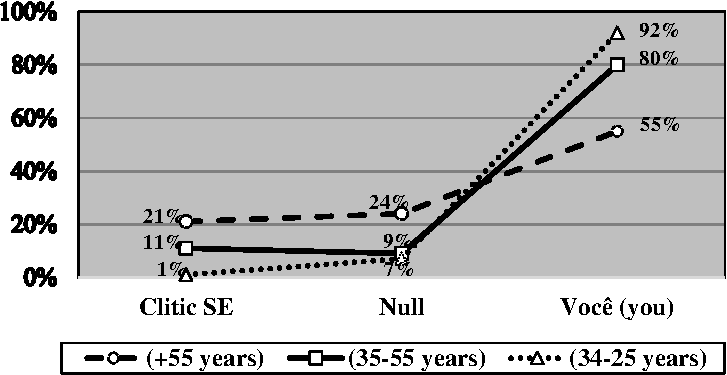
\includegraphics[width=.75\linewidth]{./img/fig3.pdf}
    \caption{Generic subjects in Brazilian Portuguese in three
    generations}\label{fig:key:26.3}
\end{figure}

Further evidence that \gls{BP}\il{Brazilian Portuguese} has become a [−NS]
language is in the fact that subject doubling (or \isi{left dislocation}) is frequent
in daily speech (cf.\ (c)).\footnote{See \citet{Britto2000}, for whom the loss
    of VS order in \gls{BP}\il{Brazilian Portuguese} made thetic sentences
    exhibit the SV order, and the categorical sentence exhibit a Left
Dislocation structure.}\newpage

\ea%45
    \label{ex:key:26.45}\ili{Brazilian Portuguese}
    \ea Eu acho que \textbf{um} \textbf{trabalho}\textbf{\tss{i}}, \textbf{ele}\textbf{\tss{i}} teria que começar por ai.\\
    \enquote*{I think that a work it would have to start from there.}
    \ex \dots{} é porque    existe uma filosofia que \textbf{o preço}\textbf{\tss{i}}\textbf{ele}\textbf{\tss{i}} tem uma paridade.\\
    \enquote*{(It)’s because (there) exists a belief     that the price (it) has a parity.}
    \z
\z

Though doubling is possible in \gls{NSL}s like \ili{Spanish}, it is inaudible because
the subject is the pronominal agreement. \gls{BP}\il{Brazilian Portuguese}, on
the other hand, pairs up with  \ili{English}, a non-NS language, with null
non-referential subjects, and their doubling is similar.

\ea%46
    \label{ex:key:26.46}
    \ea \textbf{YO\tss{i}},  com-\textbf{o}\tss{i}  pizza.
    \ex \textbf{ME}\tss{i}, \textbf{I} eat  pizza.
    \ex \textbf{EU}, [\textbf{ô}] como pizza.
    \z
\z

\citet{Roberts1993b} shows that, when \ili{French} became a [-]NS language, it
also started having subject doubling. A further subsequent change in
\ili{French} was that the “default” case of its strong pronouns changed from
nominative to dative\is{dative case}. \gls{BP}\il{Brazilian Portuguese} retained the same case
of the old strong pronouns.

\ea%47
    \label{ex:key:26.47}\ili{French}
    \ea Renars respond: \textbf{Jou, je} n’irai.
    \ex Et \textbf{jou je} cuit.
    \ex \textbf{Moi}, je le cuit.
    \z
\z

Another similarity to [-]NS languages is present in complement contexts. When
the embedded subject is a pronoun, \gls{BP}\il{Brazilian Portuguese} is exactly
like \ili{English} (EN) in anaphoric interpretation. However, its NS is
distinct in interpretation from the NS in \gls{EP}\il{European Portuguese}, a
prototypical \gls{NSL}\is{null subject languages}, and similar to the NS in
Japanese, a radical type.\is{null subject languages!radical null subject
languages}

\ea%48
    \label{ex:key:26.48}\ili{Brazilian Portuguese} = \ili{English}
    \ea {}[ John’s\tss{i} father\tss{k} ]\tss{j} said that he\tss{i/k/j} was stupid.
    \ex {}[ O pai\tss{i} do João\tss{k} ] disse que ele\tss{i/k/j} era
    estúpido.\label{ex:key:26.48b}
    \z
\z

\ea%49
    \label{ex:key:26.49} \ili{Brazilian Portuguese} $\neq$ \ili{European Portuguese}, \ili{Brazilian Portuguese} = \ili{Japanese}\\
    {}[ O pai\tss{i} do João\tss{k} ]\tss{i} disse que $\varnothing$\tss{i/*k/j} era estúpido
\z

Recall that (\ref{ex:key:26.48}b) is the form that a pre-school child would
produce, while \eqref{ex:key:26.49} is the one that may be produced  by some
Brazilians after schooling in formal settings.

\subsection{BP vs. Icelandic, a semi [−NS] language}\label{sec:key:26.3.5}

Up to now, we have been considering three types of \gls{NSL}s: the consistent,
like \gls{EP}\il{European Portuguese}, the radical\is{null subject languages!radical null subject languages} like \ili{Japanese}, and the
Partial \gls{NSL}\is{null subject languages} like Finnish. We also saw a prototypical example of a [−NS]
language, namely \ili{English}.

We have now to consider the \emph{semi pro-drop type}, like \ili{German},
namely languages that were defined as having only Null Expletives.
\citet{Biberauer2010} prefers to call these languages \emph{semi Null Subject
(semi-NS) languages.} The author considers that \emph{semi NSLs} deserve a
further division between languages like \ili{German} and \ili{Dutch}, which
have only true Null Expletives,\is{expletives} and the \ili{Icelandic} and \ili{Yiddish} type, which also
dispose of the NS with weather verbs (cf.\ also \citealt{Huang2000}).

If we consider that referential NSs in Brazilian \isi{core grammar} are [–NS]
and that it disposes of Null Expletives, we might propose that
\gls{BP}\il{Brazilian Portuguese} is actually a \textbf{semi} \textbf{[−NS]}
language, as was defended in \citet{Saab2016}, with both
\emph{quasi}-argumental  (weather verbs) and true expletive\is{expletives} NSs.

What we should point out, however, is the fact that in both types of
\emph{semi} \emph{NS} language, the expletive\is{expletives} can be overt or null
\citep{Biberauer2010}, while in Brazil there are no overt expletives, like in
consistent \gls{NSL}s.\newpage

\ea%50
    \label{ex:key:26.50ice}\ili{Icelandic}
    \ea Overt expletive\is{expletives}\\
    \gll    það rigndi í  gaer.\\
            it rains on morning\\
    \ex Null expletive\is{expletives}\\
        Í gaer rigndi  (*það).
    \z
\z

However, concerning generic null subjects, \ili{Icelandic} is exactly like
\gls{BP}\il{Brazilian Portuguese}. According to \citet{SigurdssonEgerland2009},
this language has Null Expletives and, in addition, the following generic types
of sentences: (a) \emph{generic}, like generic \ili{English} \emph{you;} (b)
\emph{arbitrary}, like \ili{English} \emph{they;} and \emph{Specific} often
referring to the speaker or a group including the speaker.

\ea%50
    \label{ex:key:26.50}\ili{Icelandic}
    \ea
	\gll	Í pessari      fjölskyldu drekkuv      pú bara ekki áfengi\\
			in this      family  may.\Tsg{}  you just not alcohol\\
	\glt	\enquote*{In this family, you just do not drink alcohol.}
    \ex
	\gll	Þeir           segja     að það rigni á morgun.\\
			they.masc say.\Tpl{} that it rains on morning\\
	\glt	\enquote*{They say it is going to rain tomorrow.}
    \ex
	\gll	Menn náðu bófanum um kvöldið.\\
			men cought.\Tpl{} culprit.the in evening.\\
	\glt	\enquote*{They caught the culprit in the evening.}
    \z
\z

\gls{BP} can have exactly the same type of generic/arbitrary NSs:

\ea%51
    \label{ex:key:26.51}\ili{Brazilian Portuguese}
    \ea
    \gll    Ali $\varnothing$ não chega  em 30 minutos\\
            there {} not arrives in 30 minutes\\
    \ex
    \gll    Na nossa familia $\varnothing$ não bebe pinga.\\
            in   our family {}       not drinks brandy\\
    \ex
    \gll    Eles dizem que $\varnothing$  vai  chover  amanhã.\\
            they say  that {}   goes to.rain   tomorrow\\
    \ex
    \gll    $\varnothing$ Pegaram o culpado ontem à noite.\\
            {} they caught   the culprit  yesterday evening\\
    \z
\z

What is different with respect to \gls{BP}\il{Brazilian Portuguese} is the
variation allowed between the NS and the weak pronouns (\emph{você} and \emph{a
gente}), a possibility inexistent in \ili{Icelandic}, except in c., where we have a
null expletive\is{expletives}:

\ea%52
    \label{ex:key:26.52}\ili{Brazilian Portuguese}
    \ea
    \gll    Ali    \textbf{você} não chega em 30 minutos\\
            there you  not  arrive in 30 minutes\\
    \ex
    \gll    Na nossa familia \textbf{a gente }              não bebe pinga.\\
            in   our family {we (the folks)}  not drinks brandy\\
    \ex ---\footnotemark{}
    \ex     \textbf{Eles} pegaram o culpado ontem à noite.
    \z
\z
\footnotetext{As shown before, \gls{BP}\il{Brazilian Portuguese} allows
    personal sentences with climate verbs:

\begin{exe}
    \exi{(i)} Essas florestas tropicais chovem muito.\\
            \enquote*{These rain forests rain.\Tpl{} a lot.}
    \exi{(ii)} Todos os meus aniversários chovem, porque  eu faço aniversário em novembro.\\
            \enquote*{All the my birthdays rain.\Tpl{}, because my birthday is
            in November.}, lit. \enquote*{\dots{} I do birthday in November}
\end{exe}}

It seems, therefore, that \emph{semi} \emph{NS} languages should be split in
three types, the last of which has referential overt pronouns, Null expletives
and Null Generic subjects.

\section{Conclusions}\label{sec:key:26.4}

After examining several empirical and theoretical works related to syntactic
phenomena in Brazilian Portuguese, \citet[411]{Roberts1993b} considered that
\gls{BP}\il{Brazilian Portuguese} was in fact undergoing a series of deep
changes along the past century, which suggested parametric changes in progress.
He added that the authors’ privileged patrimony was mainly in the rich “raw
material” they worked with, combining quantitative evidence and theoretically
inspired hypotheses.

The present chapter reports on work done on the NS conducted after
\citegen{RobKat1993} edited volume, and contains a reflection about the nature
of the NS phenomenon in \gls{BP}\il{Brazilian Portuguese} in light of recent
theoretical hypotheses on the NS Parameter.

We compared \gls{BP}\il{Brazilian Portuguese} with five language types: (a) the
consistent [NS] type; (b) the radical\is{null subject languages!radical null
subject languages} [NS] type; (c) the partial [NS] type,\is{null subject languages!partial null subject languages} (d)
the [−NS] type and the semi [−NS] type.\is{null subject languages!semi null subject languages}  The comparison has led to the
following summary:

\paragraph*{(a)} except for the expletive\is{expletives} NS, \gls{BP}\il{Brazilian Portuguese}
\textbf{core} grammar has almost entirely lost any similarities with
\gls{EP}\il{European Portuguese}, a consistent \gls{NSL}\is{null subject languages};

\paragraph*{(b)} (i) generic sentences with NSs are similar to the Japanese NSs
ones, but \gls{BP}\il{Brazilian Portuguese} generic sentences resort more
frequently to personal constructions with \emph{você} and \emph{a}
\emph{gente;} (ii) Japanese \isi{raising} structures are superficially similar to the
\gls{BP}\il{Brazilian Portuguese} ones,  as in the latter they trigger
agreement, whereas in Japanese the subject gets the topic marker \emph{-wa}.

\paragraph*{(c)} (i)  \ili{Finnish} is similar to \gls{BP}\il{Brazilian
Portuguese} \textbf{written language}, in the optionality between referential
NS and overt pronouns; (ii) even  though \ili{Finnish} and
\gls{BP}\il{Brazilian Portuguese} often resort to topicalization, in
\gls{BP}\il{Brazilian Portuguese} topics are in SpecTP, triggering agreement,
while in \ili{Finnish} they seem to be in SpecFP, an A$'$-position;

\paragraph*{(d)} (i) \gls{BP}\il{Brazilian Portuguese} has no lexical
expletives or indefinite  pronouns like \emph{one}  in \ili{English}; (ii) but,
in its referential NSs, \gls{BP}\il{Brazilian Portuguese} is exactly like
\ili{English} in production and comprehension: a [−NS] language.

In conclusion, the \isi{core grammar} of \gls{BP}\il{Brazilian Portuguese} is
(i) a [−NS] language with regard to referential subjects, and (ii) a [+NS] of
the consistent type regarding Null expletives; and (iii) a [+NS] of the
radical\is{null subject languages!radical null subject languages}
type concerning the null generic subjects. As for the system of the literate
adult, it maintains the Null expletives and Null generic subjects of the core
grammar, while, with regard to referential expressions, they are partly
pronominal (DP), like in the child \isi{core grammar}, and [−NS] like \ili{English}.

\printchapterglossary{}

\section*{Acknowledgements}

This research has the support of the National Council of Research (CNPq).

We thank the editor(s) for the accurate observations and Marcello Marcelino for
his careful revision of the first draft of this chapter.

%We are indebted to Marcello Marcelino for his careful review of the first
%version and to our anonymous reviewers for so many important suggestions. All
%remaining shortcomings are our responsibility.

{\sloppy
\printbibliography[heading=subbibliography,notkeyword=this]
}

\end{document}
